\documentclass[lecture.tex]{subfiles}

\begin{document}

\exercice{}
%\video{https://youtu.be/blablabla}
\enonce{rdm-0016}{Flexion d’une poutre (section en T)}

\begin{center}
  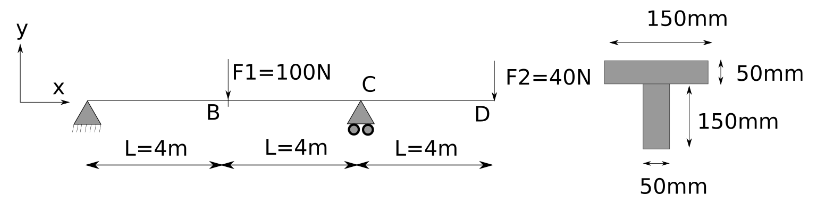
\includegraphics[scale=0.5]{exo-flexion-poutre-section-T.png}
\end{center}

\begin{enumerate}
  \item De quel type de flexion s’agit-il ?
  \item Trouver les efforts de liaison
  \item Trouver les efforts internes et tracer leurs évolutions en fonction de $x$
  \item Tracer l’évolution des contraintes $\sigma_{xx}$  en  fonction  de  $x$ pour  les  deux  surfaces hautes et basses de la poutre.
\end{enumerate}

\finenonce{rdm-0016}
\finexercice


\end{document}
